\documentclass[compress]{beamer}

%\usepackage[slantfont,boldfont]{xeCJK}
\usepackage[nofonts]{ctex}
\setCJKmainfont[ItalicFont={Kaiti SC}]{Kaiti SC}%
%\setCJKmainfont[ItalicFont={AR PL KaitiM GB}]{AR PL KaitiM GB}%
%\setCJKsansfont{WenQuanYi Zen Hei}% 文泉驿的黑体

\mode<beamer>
{
     \useinnertheme{rectangles}
     %\useoutertheme{infolines}
     %\useoutertheme{split}
     \usecolortheme{rose}
     \usecolortheme{seahorse}

     \setbeamertemplate{navigation symbols}{}%remove navigation symbols

     %\expandafter\def\expandafter\insertshorttitle\expandafter{%
     %\insertshorttitle\hfill%
     %\insertframenumber\,/\,\inserttotalframenumber}
     %\raisebox{-1ex}{
\includegraphics[width=3ex]{Overlays/logo.pdf}}}
    \setbeamertemplate{footline} {
      \leavevmode%
      \hbox{%
      \begin{beamercolorbox}[wd=.1\paperwidth,ht=2.25ex,dp=1ex,left]{date in head/foot}%
        \usebeamerfont{date in head/foot}%
        \hspace*{1ex}\raisebox{-0.8ex}{
\includegraphics[width=3ex]{Overlays/logo.pdf}}%
      \end{beamercolorbox}%
      \begin{beamercolorbox}[wd=.4\paperwidth,ht=2.25ex,dp=1ex,right]{date in head/foot}%
        \usebeamerfont{date in head/foot}\insertsection\hspace*{1ex}
      \end{beamercolorbox}%
      \begin{beamercolorbox}[wd=.4\paperwidth,ht=2.25ex,dp=1ex,left]{date in head/foot}%
        \usebeamerfont{date in head/foot}\hspace*{1ex}\insertsubsection
      \end{beamercolorbox}%
      \begin{beamercolorbox}[wd=.1\paperwidth,ht=2.25ex,dp=1ex,right]{date in head/foot}%
        \insertframenumber{} / \inserttotalframenumber\hspace*{1ex}
      \end{beamercolorbox}}%
      \vskip0pt%
    }
}


\mode<handout>
{
	\usetheme{default}
	\usepackage{pgfpages}
	\pgfpagesuselayout{4 on 1}[a4paper,landscape,border shrink=5mm]
}


\usepackage{amsmath,latexsym,amssymb,amsfonts,amsbsy}
\usepackage{graphicx}
\usepackage{hyperref}
\usepackage{textpos}
\usepackage{comment}
\usepackage{fancyvrb}
\fvset{frame=single, numbers=left, fontsize=\small}
\usepackage{tikz}
\usetikzlibrary{calc,arrows.meta, graphs, trees, shapes, positioning, automata,
shapes.geometric, shapes.multipart, er, patterns, decorations.markings, intersections, decorations.text}
\usepackage{tikz-uml}


\newcommand{\romannumber}[1]{{\textrm{\uppercase\expandafter{\romannumeral
#1}}}}

\graphicspath{{figure/}}

 
%%%%%%%%%%%%%%%%%%%%%%%%%%%%%%%%%%%%%%%%%%%%%%%%%%%%%%%%%%%%%%%%%
%    body                                                       %
%%%%%%%%%%%%%%%%%%%%%%%%%%%%%%%%%%%%%%%%%%%%%%%%%%%%%%%%%%%%%%%%%


\begin{document}

\AtBeginSection[]
{ 
    \begin{frame}<beamer> 
		\frametitle{内容提要} 
		\tableofcontents[currentsection,currentsubsection,
        subsectionstyle=show/shaded/hide] 
	\end{frame} 
} 

					
\title{第二章 ~~ 不同的分析与设计方法}

\author[面向对象的分析与设计]
{曹东刚\\\href{mailto:caodg@pku.edu.cn}{caodg@pku.edu.cn}}

\institute[北京大学]{北京大学信息学院研究生课程 - 面向对象的分析与设计 }

\date{}

\titlegraphic{
\includegraphics[height=0.10\textwidth]{Overlays/logo.pdf}}

%\includeonlyframes{current}

\begin{frame}[plain]
	\titlepage
\end{frame}

\setcounter{framenumber}{0}


\section{建模方法}

\subsection{传统方法}

\begin{frame}
\frametitle{功能分解}

\begin{columns}[c]
\column{.5\hsize}
\begin{block}{功能分解}
以系统功能为中心来组织系统
\begin{itemize}
\item 定义各种功能, 层层分解为子功能,直到可给出明确的定义
\item 根据功能/子功能的需要设计数据结构
\item 定义功能/子功能间的接口
\end{itemize}
\end{block}
\column{.5\hsize}

%\centering\includegraphics[width=0.9\hsize]{func-decom.pdf}

\begin{tikzpicture}
  [every node/.style={draw, rectangle, inner sep=1pt},
   edge from parent/.style={-Stealth, draw}]
  \node {系统}
    child {node {功能}}
    child {node {功能}
      child {node {子功能}}
      child {node {子功能}
        child {node {子功能}}
        child {node {子功能}
        edge from parent node [red, draw=none] {分解}
        }
        child {node {子功能}}
      }
      edge from parent node [red, draw=none] {分解}
    }
    child {node {功能}};
\end{tikzpicture}

\end{columns}
\end{frame}

\begin{frame}
\frametitle{功能分解得到的系统模型: 模块+接口}
%\begin{center}
%\centering\includegraphics[width=0.5\hsize]{modules.pdf}
%\end{center}
\begin{tikzpicture}
  [every node/.style={draw, rectangle, align=center, text width=1cm, inner sep=2pt}]
  \node (a) {功能模块} ;
  \node [right=2 cm of a] (ar) {功能模块} ;
  \node [below left=of a] (bl) {功能模块} ;
  \node [below =of a] (b) {功能模块} ;
  \node [below =of b] (c) {功能模块} ;
  \node [right =of c] (cr) {功能模块} ;
  \node [above right=0.5 cm of cr] (crr) {功能模块} ;
  \node [below =of c] (d) {功能模块} ;
  \node [left =of d] (dl) {功能模块} ;
  \node [right =2cm of d] (dr) {功能模块} ;

  \path[-Stealth] (a) edge (ar)
                edge (b)
                edge (bl)
            (b) edge [Stealth-Stealth](c)
                edge (bl)
                edge (cr)
                edge (crr)
                edge (dl)
            (c) edge (d)
                edge (dl)
                edge (dr)
                edge (cr)
            (bl) edge (dl)
            (d) edge (dl)
                edge (dr)
            (ar) edge (crr)
            (crr) edge (dr)
        ;
\end{tikzpicture}
\end{frame}

\begin{frame}
\frametitle{功能模块与复杂性、Bug的关系}

复杂性来源: 模块内, 模块间

\begin{center}
\centering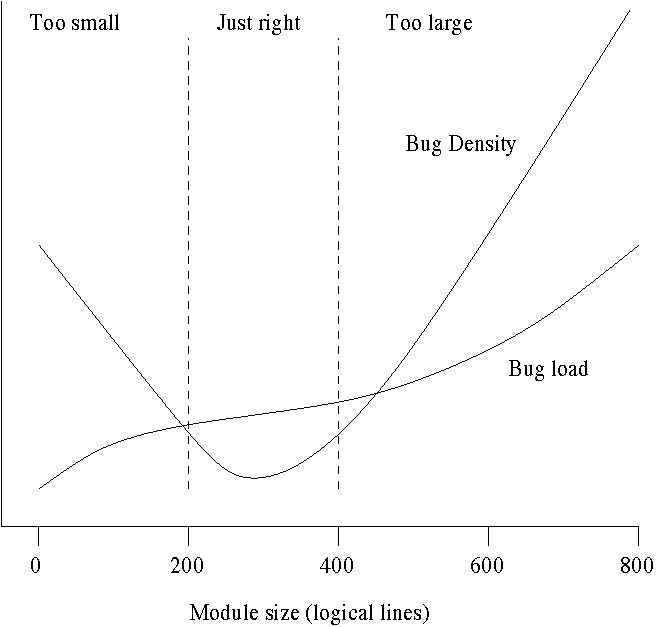
\includegraphics[width=0.65\hsize]{modulesize.pdf}
\end{center}
\end{frame}


\begin{frame}
\frametitle{功能分解的特点}
\begin{itemize}
\item \textcolor{blue}{代表软件工程问世前后人们对软件开发的朴素理解}
\item \textcolor{blue}{直接地反映用户的需求,所以工作很容易开始}
\item \textcolor{blue}{分析阶段的概念(功能)和设计阶段的概念(模块)容易对应}
\item 不能直接地映射问题域,很难检验结果的正确性
\item 对需求变化的适应能力很差, 因为功能是最易变的
\item 局部的错误和修改很容易产生全局性的影响
\end{itemize}

\end{frame}

\begin{frame}
    \frametitle{功能分解与面向对象}

功能分解的一些思想,为后来的面向对象思想吸收 \\

两种模块化方法: 

\begin{itemize}
    \item 对要完成的功能的执行过程的抽象
    \item 信息隐藏
\end{itemize}

\end{frame}




\begin{frame}
\frametitle{结构化方法: 结构化分析 + 结构化设计}
\begin{block}{结构化分析: Structured Analysis, SA}
又称数据流法,其基本策略是跟踪数据流,即研究问题域中数据如何流动,以及在各个环节上进行何种处理,从而发现数据流和加工

得到的分析模型是数据流图(DFD),主要模型元素是数据流、加工、文件及端点,外加处理说明和数据字典
\end{block}
\end{frame}

\begin{frame}
\frametitle{数据流图: Data Flow Diagram}
%\begin{center}
%\centering\includegraphics[width=0.9\hsize]{dataflow.pdf}
%\end{center}
\begin{tikzpicture}
\renewcommand{\baselinestretch}{0.8}
\tikzstyle{Ellipse}=[draw, ellipse, text width=0.8cm, minimum height=0.6cm]
\umlstateinitial[name=initial]
\umlstatefinal[x=9, y=-5, name=final]
\node [below=0.1cm of initial] {起点};
\node [below=0.1cm of final] {终点};

\node[Ellipse] (P1) at (2.5, -1) {} ;
\node[Ellipse] (P3) at (6.5, -4) {} ;
\node[Ellipse] (P2) at (4.5, -2.5) {加工} ;
\node[Ellipse] (P4) at (3, -3.5) {} ;
\node[Ellipse] (P5) at (6, -1.5) {} ;

\node [cylinder, shape border rotate=90, shape aspect=0.3, draw] (File) at (4.5, -5.5) {文件} ;  

\node [rectangle, draw, minimum height=1.5cm, align=center, blue] (Notes) at (0, -5) {处理说明 \\ ------ \\ ------} ;

\node [rectangle, draw, minimum height=1.5cm, align=center, blue] (Dict) at (8, 0) {数据词典 \\ ------ \\ ------} ;

\path[-Stealth] (initial) edge (P1)
    (P1) edge [bend right=30] node [above, sloped] {数据流} (P4) 
        edge [bend left=30] (P2)
        edge [bend left=30] node (N1) {} (P5)
    (P4) edge [bend right=10] (P2)
        edge [bend right=30, red] (File)
    (P2) edge [bend left=10] (P3)
    (P5) edge [bend left=30] node (N2) {} (P3)
    (File) edge [bend right=10, red] (P3)
    (P3) edge (final) ;
\path[thick, dotted, blue, shorten <=2pt] (Notes) edge [shorten >= 2pt] (P1)
         edge [shorten <= 2pt] (P4) 
    (Dict) edge [shorten <=2pt] (N1)
        edge [shorten <=2pt] (N2);
\end{tikzpicture}
\end{frame}

\begin{frame}
\frametitle{结构化设计: Structured Design, SD}
与功能分解法基本相同,基于模块的概念建立设计模型,分为概要设计和详细设计
\begin{itemize}
\item 概要设计:确定系统中包含哪些模块以及模块之间的调用关系,得到模块结构图(MSD)
\item 详细设计:描述每个模块内部的数据结构和操作流程
\end{itemize}
\end{frame}

\begin{frame}
\frametitle{结构化方法的特点}
\begin{itemize}
\item \textcolor{blue}{有严格的法则,强调研究问题域}
\item 仍然是间接映射问题域,难以检验分析的正确性
\item 与结构化设计的概念不一致,从分析到设计的过渡比较困难
\item 数据流和加工的数量太多,引起分析文档的膨胀,导致设计人员和设计人员理解不一致
\end{itemize}

\end{frame}

\begin{frame}
    \frametitle{结构化设计与面向对象}

    结构化设计的要点: \\

    \begin{itemize}
        \item 高内聚(cohesion)
        \item 低耦合(coupling)
    \end{itemize}

    最好的达到高内聚的方法,是从\textbf{问题域},而不是解空间中,寻找依
    据。后来的面向对象方法采纳了该思想。

\end{frame}

\begin{frame}
\frametitle{信息建模法: information modelling}
\begin{block}{信息建模法}
由实体-关系法(E-R方法)发展而来,核心概念是实体和关系
\begin{itemize}
\item 实体描述问题域中的事物,包含一组对事物数据属性的描述
\item 关系描述事物之间在数据方面的联系,有自己的属性
\item 发展之后的方法也把实体称作对象,并使用了类型和子类型的概念,作为实体(对象)的抽象描述
\end{itemize}
\end{block}
\end{frame}

\begin{frame}
\frametitle{信息模型}
%\begin{center}
%\centering\includegraphics[width=0.9\hsize]{informationm.pdf}
%\end{center}

\only<1> {
\begin{tikzpicture}
  \node[entity, minimum width=1.2cm] (E1)  at (-3,0)  {实体}
     child {node  [key attribute] {属性}}
     child {node  [attribute] {属性}};
  \node[entity, minimum width=1.2cm] (E2)  at (3,0)   {实体}
     child {node  [key attribute] {属性}} ;
  \node[relationship] at (0, 0) {关系}
     child {node  [key attribute] {属性}}
    edge node [above] {$m$} (E1)
    edge node [above] {$n$} (E2);

\node at (0, -3) {E-R图} ;
\end{tikzpicture}
}

\only<2> {
\begin{tikzpicture}
\node [diamond, aspect=1, draw, text width=2cm] (Rel) {} ;

\path (Rel.west) edge node [above] {关系} 
      node [below] {属性} (Rel.east) ;

\node [rectangle split, rectangle split parts=2, draw, text width=1cm, inner sep=10pt, align=center, left=2cm of Rel] (O1)  {对象 \nodepart{two} 属性} ;

\node [rectangle split, rectangle split parts=2, draw, text width=1cm, inner sep=10pt, align=center, right=2cm of Rel] (O2) {对象 \nodepart{two} 属性} ;

\path (Rel) edge node [above] {$n$} (O2)
    edge node [above] {$m$} (O1) ;

\node at (0, -3) {信息模型} ;
\end{tikzpicture}

}
\end{frame}


\begin{frame}
\frametitle{信息建模方法的特点}
\begin{itemize}
\item \textcolor{blue}{从问题域中的具体事物出发认识问题域,系统模型对问题域的映射比功能分解法和数据流法更直接}
\item 与面向对象方法相比,是半直接映射
\begin{itemize}
\item 强调的重点是信息建模和状态建模,而不是对象建模
\item 没有把对实体属性所进行的操作封装到实体对象中
\item 只有属性的继承,不支持操作的继承
\item 没有采用消息通讯
\end{itemize}
\end{itemize}

\end{frame}

\subsection{对象方法}

\begin{frame}
  \frametitle{面向对象方法: 面向对象的分析 + 面向对象的设计}
  \begin{itemize}
    \item 面向对象方法把问题域中的事物抽象为对象,以对象作为系统的基本构成单位
    \item 对象的属性和操作刻画了事物的静态特征和动态特征,完整地刻画了问题域中事物
    \item 对象间的继承、聚合、关联、消息等关系,如实地表达了问题域中事物之间的各种关系,符合人类的日常思维,使系统的复杂性得到控制
    \item 得到的系统模型可以直接映射问题域
  \end{itemize}
\end{frame}

\begin{frame}
\frametitle{面向对象方法和其他方法的比较}
\begin{center}
\centering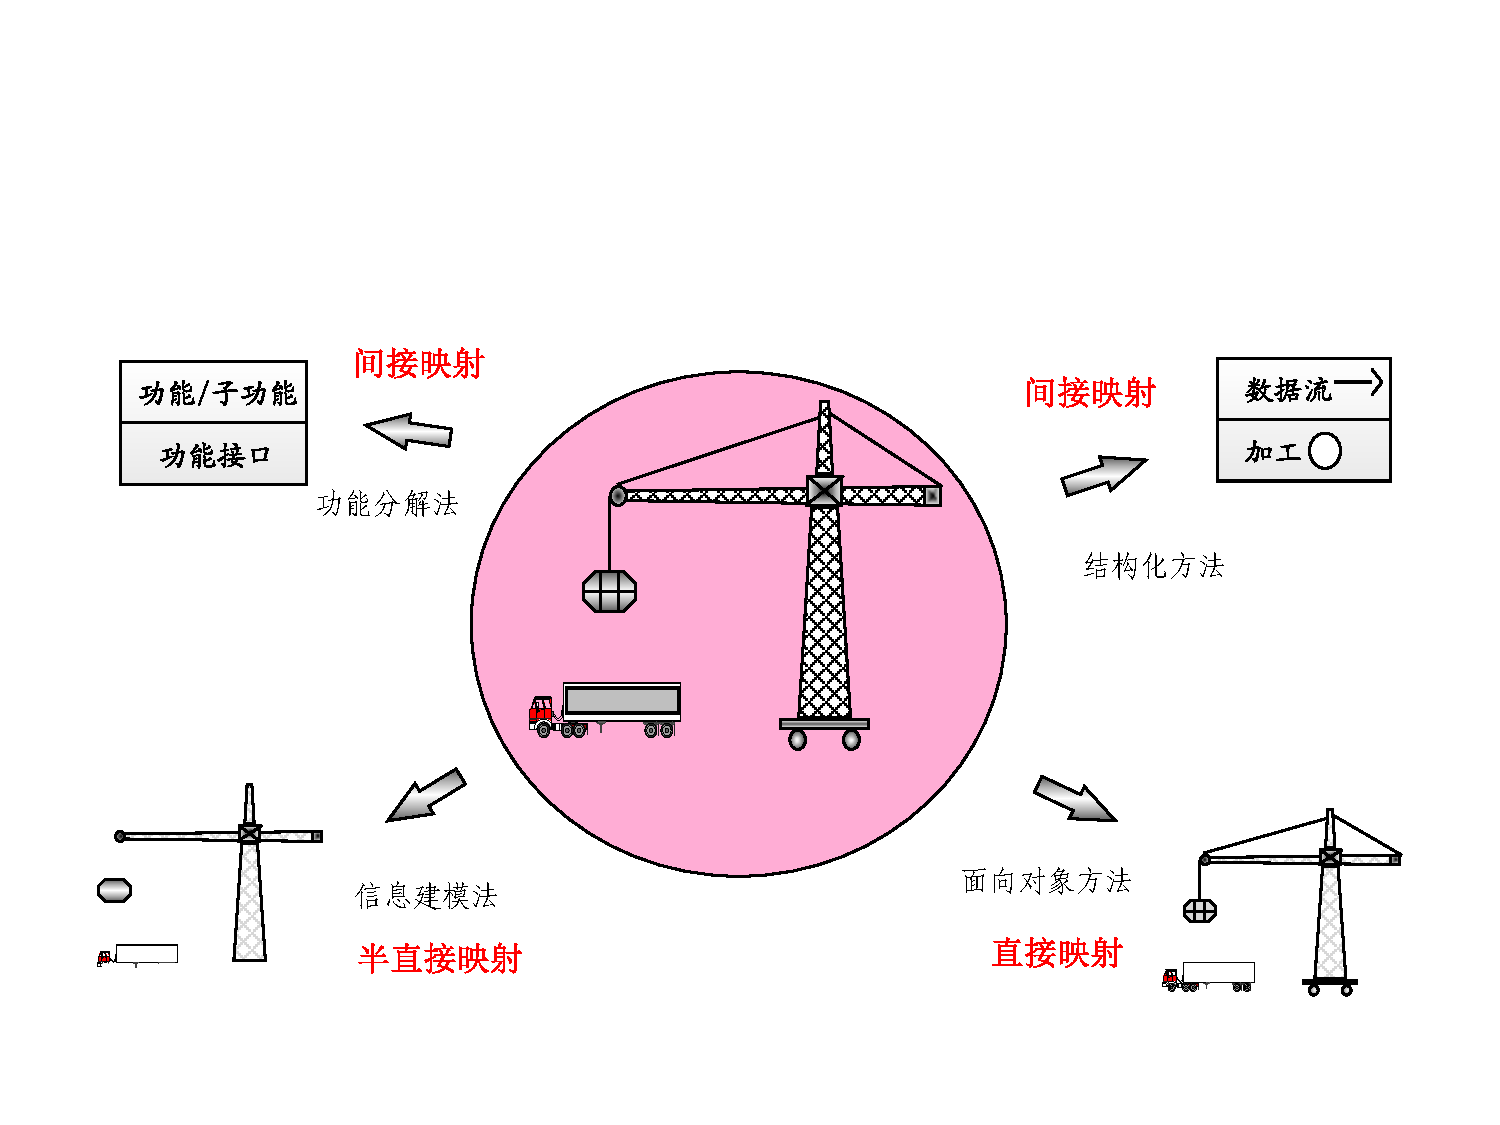
\includegraphics[width=1.0\hsize]{mapping.pdf}
\end{center}
\end{frame}

\begin{frame}
\frametitle{OO vs 结构化: 数据流和加工}

\noindent\scalebox{0.8}{
\begin{tikzpicture}
\tikzstyle{Ellipse}=[draw, ellipse, text width=0.8cm, minimum height=0.6cm]

\umlstateinitial[name=initial]
\umlstatefinal[x=13.5, name=final]
\node[Ellipse, right=1cm of initial] (P1) {登记} ;
\node[Ellipse, right=1.5cm of P1] (P2) {审批} ;
\node[Ellipse, right=1.5cm of P2] (P3) {安装} ;
\node[Ellipse, right=1.5cm of P3] (P4) {开通} ;

\node [cylinder, shape border rotate=90, shape aspect=0.3, draw] (File) 
  at (6.5, -2) {文件} ;  

\path[-Stealth] (initial) edge node [above=0.5cm] {用户信息} (P1)
  (P1) edge node [above=0.5cm] {用户登记表} (P2)
  (P2) edge node [above=0.5cm] {用户登记表} (P3)
  (P3) edge node [above=0.5cm] {用户登记表} (P4)
  (P4) edge (final) ;
\path[Stealth-Stealth] (File) edge node [below, sloped]{用户登记表}  (P1)
    edge (P2)
    edge (P3)
    edge node [below, sloped]{用户登记表} (P4) ;
\end{tikzpicture}
}
%\begin{center}
%\centering\includegraphics[width=1.0\hsize]{structured.pdf}
%\end{center}
\begin{itemize}
\item 不直接映射问题域,与问题域事物相关的数据和操作不是围绕这些事物来组织的,而是分散在数据流和加工中
\item 信息膨胀,模型中的多个数据流实现中可能只是一项数据
\item 分析模型难以与设计模型及源程序对应
\end{itemize}

\end{frame}

\begin{frame}
\frametitle{OO vs 结构化: 对象及其关系}
%\begin{center}
%\centering\includegraphics[width=.85\hsize]{oo.pdf}
%\end{center}
\scalebox{0.8}{
\begin{tikzpicture}
\renewcommand{\baselinestretch}{1.0}
\tikzumlset{fill class=white}

\umlclass{用户登记表}{用户名\\登记人\\审批人\\施工队\\号码}{登记\\
  审批 \\ 安装 \\ 开通}

\umlsimpleclass[x=-4, y=1] {营业员}
\umlsimpleclass[x=-4, y=-1] {主管人}
\umlsimpleclass[x=4, y=1] {施工队}
\umlsimpleclass[x=4, y=-1] {机房}

\umlsimpleclass[y=-4]{用户}
\umlsimpleclass[x=3, y=-4]{账单}
\umlsimpleclass[x=6, y=-4]{账单项}

\umlsimpleclass[x=-1.5, y=-6]{个人用户}
\umlsimpleclass[x=1.5, y=-6]{团体用户}

\umlVHVinherit{个人用户}{用户}
\umlVHVinherit{团体用户}{用户}

\umlassoc[mult1=1, mult2=*]{用户}{用户登记表}
\umlassoc[arg1=1, arg2=*, anchor2=141]{营业员}{用户登记表}
\umlassoc[mult1=1, mult2=*, anchor2=39]{施工队}{用户登记表}

\umldep[stereo=call, anchor2=219]{主管人}{用户登记表}
\umldep[stereo=call, anchor2=-39]{机房}{用户登记表}

\umldep[stereo=call]{营业员}{用户登记表}
\umldep[stereo=call]{施工队}{用户登记表}
\umldep[stereo=call]{机房}{账单}

\umlassoc[mult1=1, mult2=*]{用户}{账单}
\umlaggreg[mult1=1, mult2=*]{账单}{账单项}

\end{tikzpicture}
}
\end{frame}

\begin{frame}
\frametitle{面向对象分析OOA}
\begin{itemize}
\item 定义:OOA是软件生存周期的一个阶段,具有一般分析方法共同具有的内容、目标及策略;但是,它强调运用面向对象方法进行分析,用面向对象的概念和表示法表达分析结果
\item 任务:运用面向对象的概念对问题域进行分析和理解,将问题域中与\textcolor{red}{\textbf{系统责任}}有关的事物抽象为系统中的类和对象,定义其属性与操作,以及它们之间的各种关系
\item 目标:建立一个满足用户需求、直接映射问题域的OOA模型及其规约
\end{itemize}
\end{frame}

\begin{frame}
\frametitle{面向对象设计OOD -- 早期}
\begin{itemize}
\item 不是基于OOA的,大多基于结构化分析结果
\item 是OO编程方法的延伸,多数方法与编程语言有关,特别受Ada影响很大
\item 不是纯OO的,对某些OO概念(如继承)缺少支持,
搀杂一些非OO 概念(如数据流、包、模块等)
\item 不是只针对软件生存周期的设计阶段,
涉及一些系统分析问题(如识别问题域的对象)
\end{itemize}
\end{frame}

\begin{frame}
\frametitle{面向对象设计OOD -- 现今}
\begin{itemize}
\item 以OOA为基础,一般不依赖结构化分析
\item 和OOA方法构成一种共同方法体系,采用一致的概念与原则,但分属软件生存周期的不同阶段,有不同的目标及策略
\item 较全面地体现面向对象方法的概念与原则
\item 大多数方法独立于编程语言
\end{itemize}
\pause
\begin{block}{面向对象设计OOD}
就在是OOA模型基础上运用面向对象方法进行系统设计,产生一个符合具体实现条件的OOD模型
\end{block}
\end{frame}

\begin{frame}
\frametitle{软件建模面临的挑战: 问题域和系统责任的复杂性}
随着硬件性能的提高和价格的下降,软件系统所面临的问题域和系统责任越来越复杂,因此系统也越来越庞大
\begin{columns}[c]
\column{.45\hsize}
\begin{block}{问题域(problem domain)}
所开发系统的应用领域,即业务范围
\end{block}
\begin{block}{系统责任(system responsibilities)}
所开发系统应该具备的职能
\end{block}
\column{.55\hsize}
\begin{center}
\centering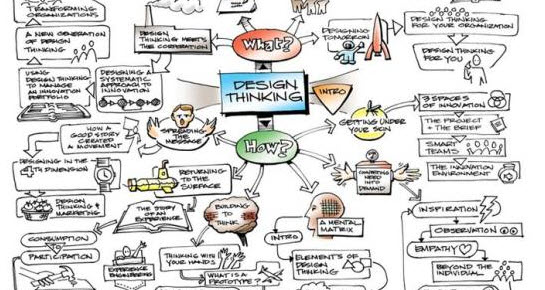
\includegraphics[width=1.0\hsize]{Design-Thinking.jpg}
\end{center}
\end{columns}
\end{frame}

\begin{frame}
\frametitle{软件建模面临的挑战: 交流问题}
\begin{itemize}
\item 软件系统的开发需要各类人员之间频繁交流,领域的多样性使软件工程中的交流问题比其他工程更为突出 
\item 有效的交流需要一种彼此都能理解的共同语言,否则将使彼此的思想难以沟通,很容易隐藏下许多错误
\end{itemize}
\begin{center}
\centering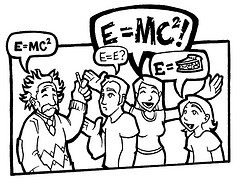
\includegraphics[width=0.4\hsize]{emc.jpg}
\end{center}
\end{frame}

\begin{frame}
\frametitle{软件建模面临的挑战: 需求变化}
开发者须接受和适应需求变化: 用户、竞争、经费等因素\ldots \\[2ex]

\begin{columns}[t]
\column{.6\hsize}
%\begin{center}
%\centering\includegraphics[width=0.9\hsize]{requirementchange.pdf}
%\end{center}

\noindent\scalebox{0.9}{
\begin{tikzpicture}
\tikzstyle{Node}=[draw, rectangle, rounded corners, align=center]
\node [Node, text width=1cm] (Req) {需求变化} ;
\node [Node, text width=1.5cm, right=of Req] (M1) {系统局部修改} ;
\node [Node, text width=1.5cm, below=of Req, xshift=1cm] (Err) {产生新错误} ;
\node [Node, text width=1.8cm, right=of Err] (M2) {受影响部分修改} ;
\node [Node, text width=1.5cm, below=of Err] (Post) {延长开发时间} ;

\path[-Stealth, blue, thick] (Req) edge [bend left=10] (M1) 
  (M1.east) edge [bend left=30] (M2.north) 
  (M2.west) edge [bend left=10] (Err.east)
  (Err.north) edge [bend left=30] (M1.west) 
  (M2.south) edge [bend left=30] (Post.east) 
  (Post.west) edge [bend left=45] (Req.west) 
 ;
\end{tikzpicture}
}
\column{.4\hsize}
\begin{itemize}
\item 功能:最易变
\item 外部接口:很易变
\item 属性:较易变
\item 对象:较稳定
\end{itemize}
\end{columns}
\end{frame}

\begin{frame}
\frametitle{软件建模面临的挑战: 复用}
复用级别提高——分析结果复用,要求分析模型的基本成分可以在多个系统中复用,
要求一个分析模型可以在多种条件下设计和实现
\begin{center}
\centering
\includegraphics[width=0.5\hsize]{softwarereuse.png}
\end{center}
\end{frame}

\begin{frame}
\frametitle{面向对象方法的优势}
\begin{itemize}
\item 对问题域和系统责任的复杂性具有较强的处理能力
\begin{itemize}
\item 系统模型能直接地映射问题域
\end{itemize}
\item 对需求的变化具有较强的适应性
\begin{itemize}
\item 按封装原则把系统中最容易变化的因素隔离起来
\end{itemize}
\item 为实现分析与设计级别的软件复用提供了有力支持
\begin{itemize}
\item 封装、继承、聚合等原则,对象的完整性、独立性等
\end{itemize}

\item 提供了便于各类相关人员交流共同语言
\begin{itemize}
\item 贯穿软件生存周期全过程的、与问题域一致的概念、词汇、原则及表示法
\end{itemize}

\end{itemize}
\end{frame}

\begin{frame}
  \frametitle{几种典型的OO方法}
  \begin{block}{方法的异同}
    概念、表示法、系统模型、开发过程、可操作性、技术支持等
  \end{block}
  \begin{itemize}
    \item Booch方法
    \item Coad-Yourdon方法
    \item Jacobson方法
    \item Rumbaugh方法
    \item \ldots
  \end{itemize}
\end{frame}

\begin{frame}
\frametitle{Booch方法}
\begin{tikzpicture}[%
    edge from parent fork down
]
  \tikzstyle{every node}=[draw, rounded corners]
  \tikzstyle{edge from parent}=[thick,draw]
  \node {六种模型图} [sibling distance=6cm]
  child { node {基本图}[sibling distance=1.5cm]
      child { node {类图}}
      child { node {对象图}}
      child { node {模块图}}
      child { node {进程图}}
    }     
    child { node {补充图}[sibling distance=2cm]
      child { node {状态转移图}}
      child { node {交互图}}
    } ;
\end{tikzpicture}
\end{frame}

\begin{frame}
  \frametitle{Booch方法宏过程}
%\begin{center}
%\centering\includegraphics[width=0.8\hsize]{booch-1.pdf}
%\end{center}

\begin{tikzpicture}
\tikzstyle{RNode}=[draw, rectangle, align=center, text width=2.5cm]

\node [RNode] (N1) {建立核心需求 \linebreak(概念化)} ;
\node [RNode] (N2) at (4, 2) {开发期望行为模型(分析)} ;
\node [RNode] (N3) at (8, 0) {建立体系结构 \linebreak(分析)} ;
\node [RNode] (N4) at (7, -3) {逐渐形成实现 \linebreak(演化)} ;
\node [RNode] (N5) at (2, -3) {管理交付后的演化(维护)} ;

\node [pattern=north east lines, pattern color=blue!50, rectangle, text width=1cm, minimum height=2cm, below= 0 of N1] (S) {} ;

\path [-Stealth, very thick] (N1.north) edge [bend left=30] (N2.west) 
  (N2.east) edge [bend left=30] (N3.north) 
  (N3.south) edge [bend left=30] (N4.north) 
  (N4.west) edge [bend left=5] (N5.east) 
  (N5.west) edge [bend left=30] ([xshift=-0.5cm,yshift=0.5cm]S.south west) ;
\end{tikzpicture}
\end{frame}

\begin{frame}
  \frametitle{Booch方法微过程}
  \begin{itemize}
    \item 类图和对象图并存
  \end{itemize}
%\begin{center}
%\centering\includegraphics[width=0.8\hsize]{booch-2.pdf}
%\end{center}
\begin{tikzpicture}
\tikzstyle{RNode}=[draw, rectangle, align=center, text width=2.5cm]

\node [RNode] (N1) {识别类\linebreak 和对象} ;
\node [RNode, below right = of N1 ] (N2) {识别类和对象的语义} ;
\node [RNode, below left= of N2] (N3) {识别类和对象的关系} ;
\node [RNode, above left= of N3] (N4) {说明类和对象的接口和实现} ;

\path [-Stealth, very thick] (N1) edge [bend left=30] (N2) 
  (N2) edge [bend left=30] (N3) 
  (N3) edge [bend left=30] (N4) 
  (N4) edge [bend left=30] (N1) ; 
\end{tikzpicture}
\end{frame}

\begin{frame}
  \frametitle{Coad/Yourdon方法}
  \begin{itemize}
    \item 概念简练,过程清晰
    \item 强调概念的一致性
    \item 过程指导不够具体
  \end{itemize}
%\begin{center}
%\centering\includegraphics[width=0.9\hsize]{cordy.pdf}
%\end{center}

\vspace*{2ex}

\hspace*{-4ex}\begin{tikzpicture}
\tikzstyle{Node}=[draw, rectangle, text width=1.8cm, minimum height=2.4cm, align=center]

\node [Node] (HIC) {人机交互 \linebreak 部分  \linebreak (HIC)} ;
\node [Node, right=0 of HIC] (PDC) {问题域 \linebreak 部分  \linebreak (PDC)} ;
\node [Node, right=0 of PDC] (TMC) {任务管理 \linebreak 部分\linebreak (TMC)} ;
\node [Node, right=0 of TMC] (DMC) {数据管理 \linebreak 部分 \linebreak (TMC)} ;

\draw [very thick] (HIC.west) -- +( -0.5cm, 0) node [xshift=-2pt, anchor=east] {结构层} ;
\draw [very thick] ([yshift=1cm]HIC.west) -- +( -0.5cm, 0) node [xshift=-2pt, anchor=east] {主题层} ;
\draw [very thick] ([yshift=0.5cm]HIC.west) -- +( -0.5cm, 0) node [xshift=-2pt, anchor=east] {类及对象层} ;
\draw [very thick] ([yshift=-0.5cm]HIC.west) -- +( -0.5cm, 0) node [xshift=-2pt, anchor=east] {属性层} ;
\draw [very thick] ([yshift=-1cm]HIC.west) -- +( -0.5cm, 0) node [xshift=-2pt, anchor=east] {服务层} ;

\draw [very thick] (DMC.east) -- +( 0.5cm, 0) ;
\draw [very thick] ([yshift=1cm]DMC.east) -- +( 0.5cm, 0) ;
\draw [very thick] ([yshift=0.5cm]DMC.east) -- +( 0.5cm, 0) ;
\draw [very thick] ([yshift=-0.5cm]DMC.east) -- +( 0.5cm, 0);
\draw [very thick] ([yshift=-1cm]DMC.east) -- +( 0.5cm, 0) ;

\node [below = 0.3cm of TMC.south west] {OOD模型的5个层次和4个部分} ;
\end{tikzpicture}
\end{frame}

\begin{frame}
  \frametitle{Jacobson方法(OOSE): 用况驱动}

  \only<1> {
      %\centering\includegraphics[width=1.0\hsize]{jacobson-1.pdf}
\noindent\begin{tikzpicture}
\tikzstyle{Model}=[draw, rectangle, rounded corners]
\tikzstyle{Process}=[draw, rectangle]

\node [Process, minimum width=8cm, minimum height=4cm] (AnaP) {} ;
\node [anchor=north west, text=red] at (AnaP.north west) {分析过程} ;

\node [Process, left=1cm of AnaP.center] (Req) {需求分析} ;
\node [Process] (Rob) at (2, 0) {健壮分析} ;

\node [Model, fill=white] (RM) at (AnaP.south) {需求模型} ;
\node [Model, fill=white] (AM) at (AnaP.south east) {分析模型} ;

\draw [Latex-Latex, thick] (AnaP.west) -- +(-1, 0) node [above=0.3, Model] {需求说明} ;

\path [Latex-Latex, thick] (AnaP.west) edge (Req.west) 
    (Req.east) edge (Rob.west)
    (Rob.east) edge (AnaP.east)
    (AnaP.east) edge +(1, 0) ;

\path [thick] (RM) edge (0, 0) 
  ([xshift=-0.5cm]AM.north) edge ([xshift=-0.5cm]AnaP.east) ;

\end{tikzpicture}
  
  }

  \only<2> {
%      \centering\includegraphics[width=1.0\hsize]{jacobson-2.pdf}
\noindent\begin{tikzpicture}
\tikzstyle{Model}=[draw, rectangle, rounded corners]
\tikzstyle{Process}=[draw, rectangle]

\node [Process, minimum width=8cm, minimum height=4cm] (AnaP) {} ;
\node [anchor=north west, text=red] at (AnaP.north west) {构造过程} ;

\node [Process, left=1cm of AnaP.center] (Req) {设计} ;
\node [Process] (Rob) at (2, 0) {实现} ;

\node [Model, fill=white] (RM) at (AnaP.south) {设计模型} ;
\node [Model, fill=white] (AM) at (AnaP.south east) {实现模型} ;

\draw [Latex-Latex, thick] (AnaP.west) -- +(-1, 0) node [above=0.3, Model] {需求模型} node [below=0.3,Model] {分析模型} ;

\path [Latex-Latex, thick] (AnaP.west) edge (Req.west) 
    (Req.east) edge (Rob.west)
    (Rob.east) edge (AnaP.east)
    (AnaP.east) edge +(1, 0) ;

\path [thick] (RM) edge (0, 0) 
  ([xshift=-0.5cm]AM.north) edge ([xshift=-0.5cm]AnaP.east) ;

\end{tikzpicture}
 
  }

  \only<3> {
      %\centering\includegraphics[width=1.0\hsize]{jacobson-3.pdf}
\hspace*{-4ex}\scalebox{1.0} {
\begin{tikzpicture}
\tikzstyle{Model}=[draw, rectangle, rounded corners]
\tikzstyle{Process}=[draw, rectangle]

\node [Process, minimum width=9cm, minimum height=4cm] (Out) {} ;
\node [anchor=north west, text=red] at (Out.north west) {测试过程} ;

\node [Process] (CT) {组装测试} ;
\node [Process, left=1cm of CT] (UT) {单元测试} ;
\node [Process, right=1cm of CT] (ST) {系统测试} ;
\node [Model, fill=white, right=0.8cm of Out.south] (TM) {测试模型} ;

\draw [Latex-Latex, thick] (Out.west) -- +(-0.8, 0) node [left=0.2, Model, text width=0.8cm] (DM) {设计模型} ;

\node [Model, above=0.5cm of DM.north west, anchor= south west] {需求模型} ;
\node [Model, below=0.5cm of DM.south west, anchor= north west] {实现模型} ;

\path [Latex-Latex, thick] (Out.west) edge (UT.west) 
    (UT.east) edge node (C1) {} (CT.west)
    (CT.east) edge node (C2) {} (ST.west)
    (ST.east) edge node (C3) {} (Out.east)
    (Out.east) edge +(0.8, 0) ;

\path [thick] (TM) edge (C1.center)
  (TM) edge (C2.center) 
  (TM) edge (C3.center) ;

\end{tikzpicture}
}
 
  }

  \only<4> {
      %\centering\includegraphics[width=0.6\hsize]{4d3d.pdf}
\begin{tikzpicture}
%\draw [help lines, step=0.5] (-3,-2) grid (5,3) ;

\draw [very thick, ->] (0,0) -- (4,0) node [text=red, right] {信息} ;
\draw [very thick, ->] (0,0) -- (0, 3) node [text=red, above] {行为} ;
\draw [very thick, ->] (0,0) -- (-2,-2) node [text=red, below left] {表示} ;
\draw [very thick, ->] (0,0) -- (-1.5,1.5) node [text=blue, above] {实现环境} ;

\draw [thick, ->] (1,2) arc [start angle=90, end angle=450, radius=0.5cm] node [above] {控制对象} ;
\draw [thick] (3,1.5) arc [start angle=90, end angle=450, radius=0.5cm] node [above] {实体对象} ;

\draw [thick, fill=white] (-1,-1) circle [fill=white, radius=0.5cm] ; 

\draw [thick] (-2, -0.75) |- (-1.5,-1) ;
\draw [thick] (-2, -1.25) |- (-1.5,-1) ;
\node at (-2, -0.25) {界面对象} ;


\end{tikzpicture}
  }
\end{frame}

\begin{frame}
  \frametitle{Rumbaugh方法(OMT)}
  \begin{columns}[c]
    \column{0.5\hsize}
      %\begin{center}
      %\centering\includegraphics[width=0.6\hsize]{omt.pdf}
      %\end{center}

\begin{tikzpicture}
%\draw [help lines, step=0.5] (-2.5,-2) grid (2.5,2) ;
\draw (0,0) -- (0,-1.5) -- node [xshift=-8pt, above=0.5cm, sloped] {对象模型} (-2, -1) -- (-2,0.5) -- cycle ;
\draw (0,0) -- (2,0.5) -- (2, -1) -- node [xshift=8pt, above=0.5cm, sloped] {动态模型} (0,-1.5) ;
\draw (-2,0.5) -- (0,1) -- (2, 0.5) ;

\node at (0, 0.5) {功能模型} ;

\end{tikzpicture}
    \column{0.5\hsize}

    过程
    \begin{itemize}
      \item 分析(面向对象)
      \item 系统设计(传统方法) 
      \item 对象设计(面向对象)
      \item 实现
    \end{itemize}
    \end{columns}
    \begin{block}{特点}
      概念严谨,阐述清楚;
      过程具体,可操作性强;
      包含了许多非OO的内容,提出若干扩充概念,偏于复杂
    \end{block}
\end{frame}

\begin{frame}
  \frametitle{对象技术发展脉络}
  \begin{center}
    \centering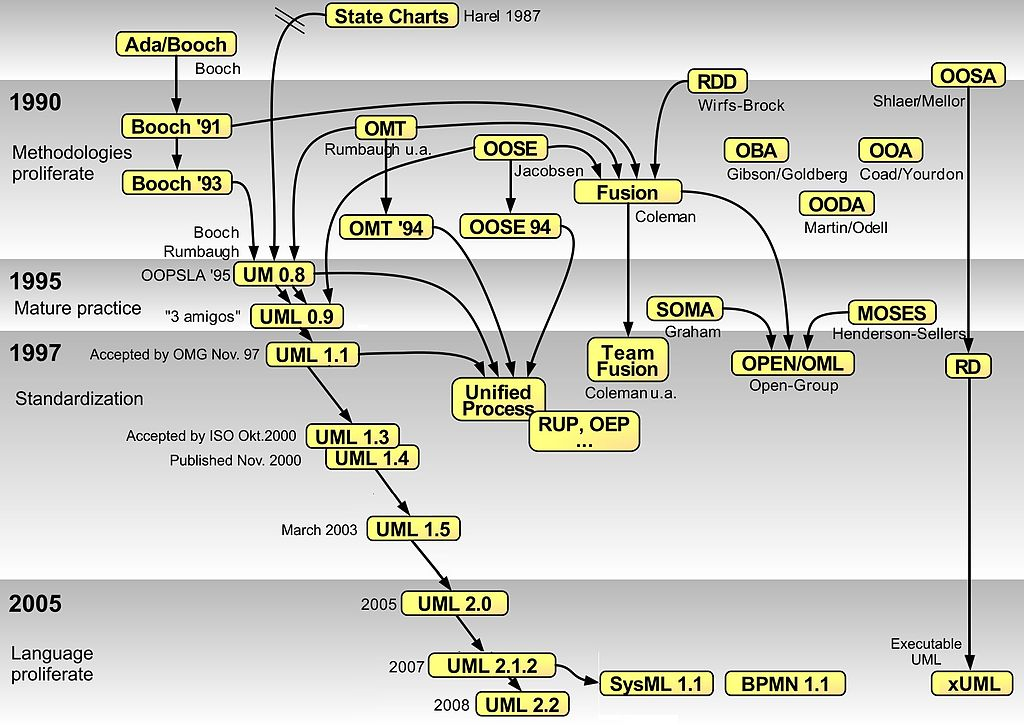
\includegraphics[width=0.9\hsize]{oo_history.jpg}
  \end{center}
\end{frame}

\section{UML}

\subsection{历史}

\begin{frame}
  \frametitle{诞生背景}
  \begin{itemize}
    \item 面向对象方法种类繁多
      \begin{itemize}
        \item 1989年约10种,1994年达到50种以上
      \end{itemize}
    \item 概念、表示法、过程策略及文档组织等方面的差异
      \begin{itemize}
        \item 使用户在选择建模方法和工具时无所适从,不利于技术交流
      \end{itemize} 

    \item 迫切需要OO概念及表示法走向统一和标准化
      \begin{itemize}
        \item 统一建模语言UML应运而生
      \end{itemize}
  \end{itemize}
\end{frame}

\begin{frame}
  \frametitle{第一阶段: OO方法学家的联合行动}
  \begin{description}
    \item [1995.10:] G. Booch与J. Rumbaugh联合, 推出Unified Method 0.8
    \item [1996.06:] I. Jacobson加入,推出UML 0.9 (Unified Modeling
      Languange)
  \end{description}
\end{frame}

\begin{frame}
  \frametitle{第二阶段: 公司的联合行动}
  \begin{description}
    \item [1996:] 成立了UML伙伴组织,12家公司加入
    \item [1997.01:] 推出UML1.0,另外5家公司加盟
    \item [1997.09:] 形成UML1.1,提交OMG作为建模语言规范提案
    \item [1997.11:] UML1.1被OMG正式采纳
  \end{description}
\end{frame}

\begin{frame}
  \frametitle{第三阶段: OMG主持下的修订}
  \begin{description}
    \item [1997-2002:] OMG成立UML修订任务组,先后产生 UML 1.2、1.3、1.4、
      1.5等版本
    \item [2000-2001:] OMG发布4个提案需求RFP,征集对UML的显著改进提案
    \item [2002-    :] 先后形成4个UML2.0规范,并继续改进
  \end{description}
\end{frame}

\begin{frame}
  \frametitle{UML是什么}
  \begin{block}{统一建模语言(UML)}
    是一种用来对软件密集型系统制品进行可
      视化、详述、构造和建档的图形语言,也可用于业务建模以及其它非软件系
      统建模
    \end{block}
    \begin{itemize}
      \item 是一种建模语言 ,不是一种建模方法
      \item 用于建立系统的分析模型和设计模型,而不是用于编程
      \item 是一种已被OMG采纳的建模语言规范(specification)
      \item 部分地采用了形式化语言的定义方式,但并不严格,不能编译执行或解释执行
    \end{itemize}

\end{frame}

\subsection{UML1}

\begin{frame}
  \frametitle{UML1主要规范}
  \begin{itemize}
    \item UML概要(UML Summary)
    \item UML语义(UML Semantics)
    \item \textbf{\textcolor{blue}{UML表示法指南}}(UML Notation Guide)
    \item UML外廓范例(UML Example Profiles)
    \item UML模型交换(UML Model Interchange)
    \item 对象约束语言 OCL (Object Constraint Language)
  \end{itemize}
\end{frame}

\begin{frame}
  \frametitle{UML1的9种模型图}
  \small
  \begin{itemize}
    \item 静态结构图(Static Structure Diagram)
      \begin{itemize}
        \item [] 类图(Class Diagram)
        \item [] 对象图(Object Diagram)
        \item [] 用况图(Use Case Diagram)
      \end{itemize}
    \item 交互图(Interaction Diagram)
      \begin{itemize}
      \item [] 顺序图(Sequence Diagram)
      \item [] 协作图(Collaboration Diagram)
      \item [] 状态图(State chart Diagrams) 
      \item [] 活动图(Activity Diagrams)
      \end{itemize}
    \item 实现图(Implementation Diagrams)
      \begin{itemize}
        \item [] 构件图(Component Diagram)
        \item [] 部署图(Deployment Diagram)
      \end{itemize}
    \end{itemize}
\end{frame}


\begin{frame}
  \frametitle{OMG四层元模型体系结构}
  %\begin{center}
    %\centering\includegraphics[width=0.9\hsize]{metam.pdf}
  %\end{center}

\hspace*{-10ex}\resizebox{!}{0.8\vsize}{
\begin{tikzpicture}
\tikzstyle{ML}=[rectangle, minimum height=1.5cm, minimum width=4.5cm, text width=4cm, align=center]
\tikzstyle{AR}=[single arrow, draw, minimum height=0.8cm, minimum width=0.2cm, text width=2ex, inner sep=1pt, text=black, fill=white, font=\scriptsize, align=center] 

\node [ML, fill=orange!50] (M3) {定义建模语言的语言 \linebreak \Large 元-元模型层} ;
\node [ML, fill=violet!20, below=0.5 of M3] (M2) {描述模型的语言 \linebreak \Large 元模型层} ;
\node [ML, fill=lime!40, below=0.5 of M2] (M1) {应用系统的抽象描述 \linebreak \Large 系统模型层} ;
\node [ML, fill=cyan!20, below=0.5 of M1] (M0) {应用领域中的事物 \linebreak \Large 应用对象层} ;

\node [left=0.2 of M3] {$M_3$} ;
\node [left=0.2 of M2] {$M_2$} ;
\node [left=0.2 of M1] {$M_1$} ;
\node [left=0.2 of M0] {$M_0$} ;

\node [AR, shape border rotate=90] at ([xshift=0.5cm, yshift=0.2cm]M2.north west) {抽象} ;
\node [AR, shape border rotate=90] at ([xshift=0.5cm, yshift=0.2cm]M1.north west) {抽象} ;
\node [AR, shape border rotate=90] at ([xshift=0.5cm, yshift=0.2cm]M0.north west) {抽象} ;

\renewcommand\baselinestretch{0.8}
\node [AR, shape border rotate=270] at ([xshift=-0.5cm, yshift=0.4cm]M2.north east) {实例化} ;
\node [AR, shape border rotate=270] at ([xshift=-0.5cm, yshift=0.4cm]M1.north east) {实例化} ;
\node [AR, shape border rotate=270] at ([xshift=-0.5cm, yshift=0.4cm]M0.north east) {实例化} ;

\renewcommand\baselinestretch{1.0}
\node [right= 0.3 of M3, text width=7cm] {元-元模型(meta-metamodel):元模型的基础体系结构,定义一种说明元模型的语言。\textcolor{blue}{例如:MOF}} ;

\node [right= 0.3 of M2, text width=7cm] {元模型(metamodel):元-元模型的一个实例,定义一种说明模型的语言。\textcolor{blue}{例如:UML}} ;

\node [right= 0.3 of M1, text width=7cm] {模型(model):元模型的一个实例,定义一种语言来描述信息领域。 \textcolor{blue}{例如:教学管理系统中的教室类、学生类、课程类}} ;

\node [right= 0.3 of M0, text width=7cm] {用户对象(user object):模型的一个实例,定义一个特定的信息领域。\textcolor{blue}{例如:一个学校——某老师,某学生,某课程}} ;




\end{tikzpicture}
}

\end{frame}

\begin{frame}
  \frametitle{抽象元类与具体元类}
  %\begin{center}
    %\centering\includegraphics[width=0.95\hsize]{metaclass-l2.pdf}
  %\end{center}
\hspace*{-5ex}\begin{tikzpicture}
\tikzumlset{fill class=white}
\umlsimpleclass{元素}
\umlsimpleclass[y=-1.5]{模型元素}
\umlsimpleclass[x=-3, y=-3]{可泛化元素}
\umlsimpleclass[x=2.5, y=-3]{关系}
\umlsimpleclass[x=-4, y=-4.5]{类目}
\umlsimpleclass[x=-7, y=-6.5, width=0.5cm]{类型}
\umlsimpleclass[x=-5.5, y=-6.5, width=0.5cm]{类}
\umlsimpleclass[x=-4, y=-6.5, width=0.5cm]{接口}
\umlsimpleclass[x=-2.5, y=-6.5, width=0.5cm]{构件}
\umlsimpleclass[x=-1, y=-6.5, width=0.5cm]{结点}

\umlsimpleclass[x=2.5, y=-6.5, width=0.5cm]{泛化}
\umlsimpleclass[x=1, y=-6.5, width=0.5cm]{关联}
\umlsimpleclass[x=4, y=-6.5, width=0.5cm]{依赖}

\umlinherit{模型元素}{元素}
\umlVHVinherit{可泛化元素}{模型元素}
\umlVHVinherit{关系}{模型元素}

\umlVHVinherit[arm2=-0.8]{类目}{可泛化元素}
\umlVHVinherit[anchor1=130, arm2=-0.8]{关联}{可泛化元素}

\umlVHVinherit[arm2=-1.3]{类型}{类目}
\umlVHVinherit[arm2=-1.3]{类}{类目}
\umlVHVinherit[arm2=-1.3]{接口}{类目}
\umlVHVinherit[arm2=-1.3]{构件}{类目}
\umlVHVinherit[arm2=-1.3]{结点}{类目}

\umlVHVinherit{关联}{关系}
\umlVHVinherit{依赖}{关系}
\umlinherit{泛化}{关系}

\draw [dashed, very thick, red] (-7, -5.2) -- (4.5,-5.2) node [at start, below, text=red, xshift=2ex] {具体元类} node [at start, above, text=red, xshift=2ex] {抽象元类};
\end{tikzpicture}
\end{frame}

\begin{frame}
  \frametitle{元模型中实例级概念引起体系结构层次的混乱}
  %\begin{center}
    %\centering\includegraphics[width=0.95\hsize]{meta-bad.pdf}
  %\end{center}

\begin{tikzpicture}[every node/.style={draw, rectangle, minimum width=1cm}]
\node (M2Assoc) {关联} ;
\node [right=of M2Assoc] (M2Class) {类} ;
\node [right=of M2Class] (M2Obj) {对象} ;
\node [right=of M2Obj] (M2Link) {链} ;

\node [below=1 of M2Class] (M1Graph) {课程:图论} ;
\node [right=2 of M1Graph] (M1Mary) {教师:玛丽} ;
\node [below left=1 of M1Graph] (M1Course) {课程} ;
\node [right=3 of M1Course] (M1Teacher) {教师} ;

\node [below=1.5 of M1Course] (M0C) {课程:计算概论} ;
\node [below=1.5 of M1Teacher] (M0Smith) {教师:史密斯} ;

\path [-Latex, dashed] 
  (M2Class) edge (M1Course)
            edge (M1Teacher)
  (M2Obj) edge (M1Graph)
          edge (M1Mary)
  (M2Link) edge ([xshift=-1cm]M1Mary.west)
  (M2Assoc) edge ([xshift=0.5cm]M1Course.east)
  (M1Course) edge (M0C)
  (M1Teacher) edge (M0Smith) 
  ([xshift=2cm]M1Course.center) edge ([xshift=2cm]M0C.center) ;

\path [-Latex] (M1Graph) edge (M1Mary)
  (M1Course) edge node[at start, xshift=2ex, below, minimum width=2ex, draw=none] {*} node[at end, xshift=-2ex, below, minimum width=2ex, draw=none] {1} (M1Teacher)
  (M0C) edge (M0Smith)  ;

\draw [thick, blue] (-2, -0.8) -- node [at start, above, draw=none] {$M_2$} node [at start, below, draw=none] {$M_1$} (7, -0.8) ;

\draw [thick, blue] (-2, -3.6) -- node [at start, below, draw=none] {$M_0$} (7, -3.6) ;

\end{tikzpicture}

\end{frame}

\begin{frame}
  \frametitle{扩展机制}
  \begin{block}{扩展机制}
      附加到其他模型元素之上以,将原有的建模元素特化成一种语义较特殊的新
      变种,或者表示出它们的某些细节
    \end{block}
    \begin{itemize}
      \item 约束(constraint) :用于说明某些必须保持为真的命题
      \item 注释(comment): 对模型元素的细节所进行的解释
      \item 标记值(Tagged Value):表示模型元素的附加的特征
      \item 衍型(stereotype): 附加到其他模型元素之上,从而将原有的建模元
        素定制成一种语义较为特殊的新变种
    \end{itemize}
\end{frame}

\begin{frame}
  \frametitle{衍型的表示法和例子}
  %\begin{center}
    %\centering\includegraphics[width=0.95\hsize]{stereot.pdf}
  %\end{center}

\begin{tikzpicture}
\tikzumlset{fill class=white}

\umlemptyclass{类名A}{}{}
\node [text=red, right=0.1 of 类名A] (Note) {+关键词或图标=} ;
\umlemptyclass[x=5.5, type=active]{类名B}{}{}
\umlemptyclass[x=8, type=界面]{类名C}{}{}

\end{tikzpicture}

\end{frame}

\subsection{UML2}

\begin{frame}
  \frametitle{UML2概况}
  \begin{columns}[t]
    \column{0.6\hsize}
    \begin{block}{UML Superstructure}
      提供可直接用来构造用户系统的各种模型元素,以及从不同的视角对系统进
      行建模的各种模型图
    \end{block}
    \begin{block}{UML Infrastructure}
      定义一个可复用的元语言核心,用来定义UML、MOF和CWM
      等元模型 
    \end{block}
    \column{0.4\hsize}
    \begin{block}{UML Diagram Interchange}
      给出在不同的建模工具之间实现模型交换的规范
    \end{block}
    \begin{block}{UML OCL}
      一个形式化的语言,描述模型约束信息 \\

    \end{block}
  \end{columns}
\end{frame}

\begin{frame}
  \frametitle{UML2的14种模型图}
  %\begin{center}
    %\centering\includegraphics[width=1.0\hsize]{uml2-diagrams.pdf}
  %\end{center}

\hspace*{-6ex}\scalebox{0.92}{
\begin{tikzpicture}[node distance=2cm]
\tikzstyle{abstract}=[rectangle, draw=black,
        text centered, font=\itshape \footnotesize,  anchor=north,
        text width=2cm]
\tikzstyle{diagram}=[rectangle, draw=black, 
        text centered, font=\footnotesize, anchor=north, , text width=2cm]
\tikzstyle{myarrow}=[->, >=open triangle 90, thick]
\tikzstyle{line}=[-, thick]

  \node (Diagram) [abstract, rectangle] { Diagram };
    \node (AuxNode02) [text width=0.5cm, below=1.5cm of Diagram] {};
    \node (Structure) [abstract, rectangle , left=of AuxNode02]
    { Structure \\[-1ex] Diagram};
    \node (Behaviour) [abstract, rectangle , right=of AuxNode02]
    { Behaviour \\[-1ex] Diagram };
        
    \node (AuxNode03) [below=1.5cm of Structure] {};
    \node (Profile) [diagram, rectangle , left=of AuxNode03, xshift=1cm]
    { Profile \\[-1ex] Diagram};
    \node (Component) [diagram, rectangle , right=of AuxNode03, xshift=-3cm]
    { Component \\[-1ex] Diagram};
    \node (Class) [diagram, rectangle , below=0.4cm of Profile]
    { Class \\[-1ex] Diagram };
    \node (Composite) [diagram, rectangle , below=0.4cm of Class]
    { Composite \\[-1.5ex] Structure \\[-1.5ex] Diagram };
    \node (Deployment) [diagram, rectangle , below=0.4cm of Component]
    { Deployment \\[-1ex] Diagram };
        
    \node (Package) [diagram, rectangle , right=of Component, xshift=-1.6cm]
    { Package \\[-1ex] Diagram};
    \node (Object) [diagram, rectangle , below=0.4cm of Package]
    { Object \\[-1ex] Diagram };

    \node (AuxNode04) [below=1.5cm of Behaviour] {};
    \node (Usecase) [diagram, rectangle , left=of AuxNode04, xshift=2cm]
    { Use Case \\[-1ex] Diagram };
    \node (Activity) [diagram, rectangle , right=of AuxNode04, xshift=-2cm]
    { Activity \\[-1ex] Diagram };
    \node (Interaction) [diagram, rectangle , below=0.4cm of Usecase]
    { Interaction \\[-1ex] Diagram };
    \node (State) [diagram, rectangle , below=0.4cm of Activity]
    { State Machine \\[-1.5ex] Diagram };

    \node (AuxNode05) [below=1.5cm of Interaction] {};
    \node (Timing) [diagram, rectangle , below=1.5cm of Interaction ]
    { Timing \\[-1ex] Diagram };
    \node (Sequence) [diagram, rectangle , left=0.4cm of Timing]
    { Sequence \\[-1ex] Diagram };
    \node (Communication) [diagram, rectangle , left=0.4cm of Sequence]
    { Communication \\[-1ex] Diagram };
    \node (Interover) [diagram, rectangle ,
    right=0.4cm of Timing.north east,anchor=north west]
    { Interaction \\[-1.5ex] Overview \\[-1.5ex] Diagram };

    \draw[myarrow] (Structure.north) -- ++(0,0.5) -| (Diagram.south);
   
    \draw[myarrow] (Profile.west) -- ++(-0.2,0)
        -- ([yshift=0.5cm, xshift=-0.2cm] Profile.north west)
        -| ([xshift=-0.0cm]Structure.south);
    \draw[line] (Class.west) -- ++(-0.2,0) -- ([xshift=-0.2cm] Profile.west) ;
    \draw[line] (Composite.west) -- ++(-0.2,0) -- ([xshift=-0.2cm] Profile.west) ;

    \draw[myarrow] (Component.east) -- ++(0.2,0)
        -- ([yshift=0.5cm, xshift=0.2cm] Component.north east)
        -| ([xshift=0cm]Structure.south);
    \draw[line] (Deployment.east) -- ++(0.2,0) -- ([xshift=0.2cm] Component.east) ;
    \draw[line] (Package.west) -- ++(-0.2,0) ;
    \draw[line] (Object.west) -- ++(-0.2,0) ;
    
    \draw[myarrow] (Behaviour.north) -- ++(0,0.5) -| (Diagram.south);

    \draw[myarrow] (Usecase.west) -- ++(-0.2,0)
      -- ([yshift=0.5cm, xshift=-0.2cm] Usecase.north west)
      -| ([xshift=0cm]Behaviour.south);
    \draw[line] (Interaction.west) -- ++(-0.2,0)
      -- ([xshift=-0.2cm] Usecase.west) ;

    \draw[myarrow] (Activity.east) -- ++(0.2,0)
      -- ([yshift=0.5cm, xshift=0.2cm] Activity.north east) -|
     ([xshift=-0cm]Behaviour.south);
    \draw[line] (State.east) -- ++(0.2,0)
      -- ([xshift=0.2cm] Activity.east) ;

    \draw[myarrow] (Sequence.north) -- ++(0,0.5) -| (Interaction.south);
    \draw[myarrow] (Communication.north) -- ++(0,0.5) -| (Interaction.south) ;
    \draw[myarrow] (Timing.north) -- ++(0,0.5) -| (Interaction.south) ;
    \draw[myarrow] (Interover.north) -- ++(0,0.5) -| (Interaction.south) ;
\end{tikzpicture}
}
\end{frame}

\begin{frame}
  \frametitle{学习建议}
  \begin{itemize}
    \item 重点掌握UML直接提供给应用模型开发者使用的建模元素,即“具体元类
      ”; 熟练地掌握面向对象方法最基本的概念
    \item 掌握类图、用况图、顺序图、活动图、状态机图、构件图
    \item 着眼于实际应用,从UML的复杂性中解放出来
    \item UML只是一种建模语言,\textbf{\textcolor{red}{不是建模方法}},
      它不包括过程,而且是独立于过程的
    \item 动手实践,使用工具;选择合适的项目开始实际应用
  \end{itemize}
\end{frame}

\section{本课程方法}

\begin{frame}
  \frametitle{宗旨}
  \begin{itemize}
    \item 充分运用面向对象方法的基本概念,限制扩充概念 
    \item 加强过程指导
      \begin{itemize}
        \item 给出用最基本的OO概念自然而有效地解决建模问题的策略
      \end{itemize}
    \item 强调在类的抽象层次上建立系统模型
      \begin{itemize}
        \item 所有对象的属性和操作以及对象之间的关系,都通过它们的类来描述,
          而不是针对个别对象实例进行描述
      \end{itemize}
  \end{itemize}

\end{frame}

\begin{frame}
  \frametitle{主要建模元素}
  \begin{itemize}
    \item 对象、类(所有的对象都通过类来表示) 
    \item 属性、操作(类属性和实例属性,被动操作和主动操作) 
    \item 一般-特殊关系,一般-特殊结构
    \item 整体-部分关系,整体-部分结构
    \item 关联 (二元关联、多元关联)
    \item 消息 (控制流内部的消息,控制流之间的消息)
  \end{itemize}
\end{frame}

\begin{frame}
  \frametitle{主要原则}
  \begin{itemize}
    \item 抽象: 数据抽象,过程抽象
    \item 分类
    \item 封装
    \item 继承
    \item 聚合
    \item 关联
    \item 消息通信
    \item 粒度控制
    \item 行为分析
  \end{itemize}
\end{frame}

\begin{frame}
  \frametitle{OOA模型和OOD模型}
  \begin{block}{模型: 正式理解}
    一个系统模型,应包括建模过程中产生的图形、文字等各种形式的文档。因为
    ,所谓“模型”是指某一级别上的系统抽象描述,构成这种描述的任何资料都是
    模型的一部分
  \end{block}
  \begin{block}{模型: 习惯说法}
    大部分OOA/OOD著作谈到“模型”,一般是指OOA或OOD过程中产生的图形文档 \\
    本课程采用习惯说法,将模型和模型规约分开讨论
  \end{block}

\end{frame}

\begin{frame}
  \frametitle{三种模型}
  \begin{block}{基本模型---类图}
    面向对象的建模中最重要、最基本的模型图,可从对象层、特征层、关系层看
  \end{block}
  \begin{block}{需求模型---用况图}
    用况是一项系统功能使用情况的说明。把所有参与者对系统功能
    的使用情况确切描述出来,便全面定义了系统的功能需求
  \end{block}
  \begin{block}{辅助模型---其他图}
    对类图起到辅助作用,提供更详细的建模信息,或者从不同的视角来描述系统
    。例如包图、顺序图、活动图等
  \end{block}
\end{frame}

\begin{frame}
  \frametitle{OOA模型框架}
  %\begin{center}
    %\centering\includegraphics[width=0.9\hsize]{ooa-shao.pdf}
  %\end{center}
\resizebox{0.9\hsize}{!} {%
\begin{tikzpicture}
\tikzstyle{caption}=[font=\bfseries \small, align=center]
\tikzstyle{ntext}=[font=\small, align=center]
%  \draw [help lines, step=0.5cm] (0,0) grid (8,5) ;
  \draw (0,0) rectangle (8,1) ;
  \node [caption] at (4, 0.5) {模型规约} ;
  \draw (0,1.2) rectangle (1.5,5) ;
  \node [caption] at (0.75, 4.5) {需求模型} ;
  \node [ntext] at (0.75, 2.75) {用况图} ;
  \draw (6.5,1.2) rectangle (8,5) ;
  \node (ReqT) [caption] at (7.25, 4.5) {辅助模型} ;
  \node (PkgT) [below=0.5cm of ReqT, ntext] {包图} ;
  \node (SeqT) [below=0.1cm of PkgT, ntext] {顺序图} ;
  \node (ActT) [below=0.1cm of SeqT, ntext] {活动图} ;
  \node (EtcT) [below=0.1cm of ActT, ntext] {\dots} ;
  \draw (1.7,1.2) rectangle (6.3,5) ;
  \node (ClsT) [caption] at (4, 4.5) {基本模型:类图} ;
  \node (ObjL) [below=0.5cm of ClsT, text width=2cm, minimum
  height=0.6cm, rectangle, draw, xslant=0.6] {} ;
  \node (ObjT) [below=0.5cm of ClsT, ntext] {对象层} ;
  \node (FeaL) [below=0.2cm of ObjT, text width=2cm, minimum
  height=0.6cm, rectangle, draw, xslant=0.6] {} ;
  \node (FeaT) [below=0.2cm of ObjT, ntext] {特征层} ;
  \node (ReaL) [below=0.2cm of FeaT, text width=2cm, minimum
  height=0.6cm, rectangle, draw, xslant=0.6] {} ;
  \node (ReaT) [below=0.2cm of FeaT, ntext] {关系层} ;
\end{tikzpicture}
}

\end{frame}

\begin{frame}
  \frametitle{OOD模型框架}
  %\begin{center}
  %  \centering\includegraphics[width=0.5\hsize]{ood-shao.pdf}
  %\end{center}
\begin{tikzpicture}
\renewcommand{\baselinestretch}{1.0}
%\draw [help lines, step=0.5cm] (-4,0) grid (6,6) ;

\draw [very thick] (0,0) -- (5,0) -- (5,5) -- (0,5) -- (0,0) ;
\draw (0,0) -- (1,1) -- (1,5);
\draw (5,0) -- (4,1) -- (4,5);
\draw (1,1) -- (4,1) ;
\node [text width=1pt] at (0.4,3.0) {人机交互部分} ;
\node [text width=1pt] at (4.4,3.0) {数据接口部分} ;
\node at (2.5,0.5) {控制驱动部分} ;
\node at (2.5,3.0) {\Large{问题域部分}} ;

\draw [very thick](0,0) -- (-3,1) --(-3,6) ;
\draw [name path=c2, very thick] (-3,6) -- (0,5) ;
\draw [name path=c1, postaction={decorate, decoration={text along path, raise=-15pt, text align={align=center}, text = {模型规约}}}] (-3,2) -- (0,1) ;

\draw [very thick](5,5) -- (2,6)--(-3,6) ;
\path [name path=v1] (-0.75,0) -- (-0.75,6) ;
\path [name path=v2] (-2.25,0) -- (-2.25,6) ;

\path [name intersections={of=c1 and v1,by=E1}];
\path [name intersections={of=c2 and v1,by=E2}];
\draw (E1) -- (E2) ;
\path [name intersections={of=c1 and v2,by=F1}];
\path [name intersections={of=c2 and v2,by=F2}];
\draw (F1) -- (F2) ;

\node [text width=1pt] at (-2.75, 4) { 需求模型} ;
\node [text width=1pt] at (-0.5, 3) { 辅助模型} ;
\node [text width=1pt] at (-1.75, 3.5) { \Large 类图} ;

\end{tikzpicture}
\end{frame}

\begin{frame}[plain]
  %\frametitle{OOA过程}
  %\begin{center}
  %  \centering\includegraphics[width=0.65\hsize]{ooa-process.pdf}
  %\end{center}

\hspace*{-4ex}\resizebox{!}{\vsize}{
\renewcommand{\baselinestretch}{0.8}
\begin{tikzpicture}
\tikzstyle{Snode}=[draw, rectangle, text width=1.2cm, align=center]
\tikzstyle{Bnode}=[draw, rectangle, text width=1.6cm, align=center]
\tikzstyle{Rnode}=[draw, rectangle, text width=2.5cm, align=center]
\tikzstyle{SLink}=[-{Triangle[length=4pt]}, line width=4pt, cyan] ; 
\tikzstyle{DLink}=[{Triangle[length=4pt]}-{Triangle[length=4pt]}, line width=4pt, cyan] ; 
%\draw [help lines, step=0.5] (-6,-5) grid (6,7) ;

\node [font=\Large] at (-5.5, 5) {OOA过程} ;

\draw [thick] (-4,2.5) -- (-4, 6) 
    -- node [below] {建立需求模型} (4, 6) 
    -- (4, 2.5) --cycle ;
\node [Rnode] (R3) at (0, 3) {定义用况} ;
\node [Rnode, above=0.4 of R3] (R2) {发现参与者} ;
\node [Rnode, above=0.4 of R2] (R1) {确定系统边界} ;

\path [SLink] (R1) edge (R2) 
  (R2) edge (R3) ;

\pause

\draw [thick] (-4,-1.5) -- (-4, 1.5) 
    -- node [below] {建立基本模型} (4, 1.5) 
    -- (4, -1.5) --cycle ;
\node [Bnode] (B1) at (0, 0.5) {发现对象} ;
\node [Bnode, below left=0.5 of B1] (B2) {定义对象的特征} ;
\node [Bnode, below right=0.5 of B1] (B3) {定义对象间的关系} ;

\path [DLink] (B1.east) edge [out=0, in=90]  (B3.north) 
  (B2) edge (B3) 
  (B1.west) edge [out=180, in=90] (B2.north) 
  (0, 2.5) edge (0, 1.5) ;


\pause

\draw [thick] (-4,-4.3) -- (-4, -2.5) 
    -- node [below] {建立辅助模型} (4, -2.5) 
    -- (4, -4.3) --cycle ;
\node [Snode] (A1) at (-3, -3.6) {建立\linebreak 包图} ;
\node [Snode, right=0.5 of A1] (A2) {建立\linebreak 顺序图} ;
\node [Snode, right=0.5 of A2] (A3) {建立\linebreak 活动图} ;
\node [Snode, right=0.5 of A3] (A4) {建立\linebreak 其他图} ;

\path [DLink] (0, -2.5) edge (0, -1.5) ;

\pause

\renewcommand\baselinestretch{1.2}
\node [draw, thick, rectangle, minimum width= 1cm, minimum height=5cm, text width=2ex] (Spec) at (5.5, 0) {  建立模型规约} ;

\path [SLink] (4,4) edge [out=0, in=90] (Spec.north) ;

\path [DLink] (Spec) edge (4,0) 
  (Spec.south) edge[out=270, in=0] (4, -3.5) ;

\pause

\node [draw, thick, rectangle, minimum width= 1cm, minimum height=5cm, text width=2ex] (Prot) at (-5.5, 0) {  原型开发} ;

\path [SLink] (-4,4) edge [out=180, in=90] (Prot.north) ;

\path [DLink] (Prot) edge (-4,0) 
  (Prot.south) edge[out=270, in=180] (-4, -3.5) ;


\end{tikzpicture}
}
\end{frame}

\begin{frame}
  \frametitle{OOD过程}
  %\begin{center}
    %\centering\includegraphics[width=0.7\hsize]{ood-process.pdf}
  %\end{center}
\noindent\begin{tikzpicture}[thick]
\tikzstyle{vecArrow} = [thick, decoration={markings,mark=at position
   1 with {\arrow[thin, scale=2]{open triangle 60}}},
   double distance=3pt, shorten >= 10pt,
   preaction = {decorate},
   postaction = {draw,line width=3pt, white,shorten >= 9pt}
]
\tikzstyle{Node} = [thick, rectangle, draw, minimum height=3ex, minimum width=3.5cm]

  \node (ooa) {\textcolor{blue}{输入OOA模型}};
  \node [Node, below = 1cm of ooa] (business) {问题域部分设计};
  \node [Node, below = 1cm of business] (control) {控制驱动部分设计};
  \node [Node, below = 1cm of control] (deploy) {构件化与系统部署} ;
  \node [below = 1cm of deploy] (oop) {\textcolor{blue}{向OOP输出OOD模型}} ;
  \node [Node, right = 0.5cm of control.east] (data) {数据接口部分设计};
  \node [Node, left = 0.5cm of control.west] (gui) {人机交互部分设计};

  \draw[vecArrow] (ooa) to (business);
  \draw[vecArrow] ([yshift=-1pt]business.south) to (control);
  \draw[vecArrow] ([yshift=-1pt]control.south) to (deploy);
  \draw[vecArrow] ([yshift=-1pt]deploy.south) to (oop);
  \draw[vecArrow] ([xshift=-1.0cm, yshift=-0.1cm]business.south) to ([yshift=+0.1cm]gui.north);
  \draw[vecArrow] ([xshift=+1.0cm, yshift=-0.1cm]business.south) to ([yshift=+0.1cm]data.north);
  \draw[vecArrow] ([yshift=-0.1cm]gui.south) to ([xshift=-1cm, yshift=+0.1cm]deploy.north);
  \draw[vecArrow] ([yshift=-0.1cm]data.south) to ([xshift=+1cm, yshift=+0.1cm]deploy.north);
\end{tikzpicture}

\end{frame}

\begin{frame}
  \frametitle{OOA与OOD的关系}
  一致的概念与表示法、不同的抽象层次
  \begin{block}{OOA}
    研究问题域和用户需求,运用面向对象的观点发现问题域中与系统责任有关的
    对象,以及对象的特征和相互关系。目标是建立一个直接映射问题域,符合用
    户需求的OOA模型
  \end{block}
  \begin{block}{OOD}
    在OOA模型基础上,针对选定的实现平台进行系统设计,按照实现的要求进行
    具体的设计,目标是产生一个能够在选定的软硬件平台上实现的OOD模型
  \end{block}
  
\end{frame}

\begin{frame}
  \frametitle{OOA和OOD适应各种软件生存周期模型}
  \begin{columns}[c]
    \column{0.4\hsize}
    \begin{block}{瀑布模型}
      强调严格的阶段划分和前后次序 \\
      先做完OOA再进行OOD
  \end{block}
    \column{0.6\hsize}
    %\begin{center}
      %\centering\includegraphics[width=0.8\hsize]{waterfall.pdf}
    %\end{center}
\begin{tikzpicture}
  [every node/.style={draw, thick, rectangle, text width=1.2cm, minimum height=1cm, align=center}, shorten >=1pt, shorten <=1pt]

\renewcommand{\baselinestretch}{1.0}

\node (OOA) {分析 \linebreak (OOA)} ;
\node [below =0.3 of OOA, xshift=1cm] (OOD)  {设计 \linebreak (OOD)} ;
\node [below =0.3 of OOD, xshift=1cm] (OOP) {编程 \linebreak (OOP)} ;
\node [below =0.3 of OOP, xshift=1cm] (TEST) {测试} ;
\node [below =0.3 of TEST, xshift=1cm] (MET) {维护} ;

\path [->, draw=gray, ultra thick] (OOA) edge [bend left] ([xshift=-0.3cm]OOD.north east) ;
\path [->, draw=gray, ultra thick] (OOD) edge [bend left] ([xshift=-0.3cm]OOP.north east) ;
\path [->, draw=gray, ultra thick] (OOP) edge [bend left] ([xshift=-0.3cm]TEST.north east) ;
\path [->, draw=gray, ultra thick] (TEST) edge [bend left] ([xshift=-0.3cm]MET.north east) ;


\end{tikzpicture}
\end{columns}
\end{frame}


\begin{frame}
  \frametitle{OOA和OOD适应各种软件生存周期模型}
  \begin{columns}[c]
    \column{0.5\hsize}
    \begin{block}{喷泉模型}
    各个阶段之间没有严格的界限,其活动可以交叠和回溯\\
    有些工作既可在OOA中进行,也可在OOD中进行
  \end{block}
    \column{0.5\hsize}
    %\begin{center}
      %\centering\includegraphics[width=0.6\hsize]{fountain.pdf}
    %\end{center}

\scalebox{0.9}{
\begin{tikzpicture}
  \renewcommand\baselinestretch{0.8}
  \tikzstyle{Process}=[draw, ellipse, thick, minimum width=2.5cm, minimum height=1.5 cm, text width=1cm, align=center, fill=white]
  \node [Process] (Evo) {演化} ;
  \path [->, thick] (Evo.west) edge [bend right] ++(-1, -1) ; 
  \path [->, thick] (Evo.east) edge [bend left] ++(1, -1) ; 

  \node [Process, below=0.5 of Evo] (Int) {集成} ;
  \path [->, thick] ([xshift=-1ex, yshift=-1ex]Int.north) edge [bend right] ([xshift=1ex]Int.west) ; 
  \path [->, thick] ([xshift=1ex, yshift=-1ex]Int.north) edge [bend left] ([xshift=-1ex]Int.east) ; 

  \node [Process, below=0.2 of Int.center] (Tes) {测试} ;
  \path [->, thick] ([xshift=-1ex, yshift=-1ex]Tes.north) edge [bend right] ([xshift=1ex]Tes.west) ; 
  \path [->, thick] ([xshift=1ex, yshift=-1ex]Tes.north) edge [bend left] ([xshift=-1ex]Tes.east) ; 

  \node [Process, below=0.2 of Tes.center] (OOP) {编程 \linebreak (OOP)} ;
  \path [->, thick] ([xshift=-1ex, yshift=-1ex]OOP.north) edge [bend right] ([xshift=1ex]OOP.west) ; 
  \path [->, thick] ([xshift=1ex, yshift=-1ex]OOP.north) edge [bend left] ([xshift=-1ex]OOP.east) ; 

  \node [Process, below=0.4 of OOP.center] (OOD) {设计 \linebreak (OOD)} ;
  \path [->, thick] ([xshift=-1ex, yshift=-1ex]OOD.north) edge [bend right] ([xshift=1ex]OOD.west) ; 
  \path [->, thick] ([xshift=1ex, yshift=-1ex]OOD.north) edge [bend left] ([xshift=-1ex]OOD.east) ; 

  \node [Process, below=0.4 of OOD.center] (OOA) {分析 \linebreak (OOA)} ;
  \path [->, thick] ([xshift=-1ex, yshift=-1ex]OOA.north) edge [bend right] ([xshift=1ex]OOA.west) ; 
  \path [->, thick] ([xshift=1ex, yshift=-1ex]OOA.north) edge [bend left] ([xshift=-1ex]OOA.east) ; 

  \path [->, ultra thick] (Int) edge (Evo) ;
  \path [ultra thick] ([yshift=-0.2cm]OOA.south) edge (OOA) ;

\end{tikzpicture}
}
\end{columns}
\end{frame}


\begin{frame}
  \frametitle{OOA和OOD分工的两种观点}

  关键问题:对象的特征细节在分析还是设计时定义? \\[2ex]

  \begin{columns}[c]
    \column{0.5\hsize}
    %\begin{center}
      %\centering\includegraphics[width=0.9\hsize]{2viewpoint.pdf}
    %\end{center}

\scalebox{0.9}{
\begin{tikzpicture}
\renewcommand{\baselinestretch}{1.0}
\draw [thick] (-2,-2) -- (-2,2) -- (2,2) -- (2,-2) -- cycle ;
\draw [thick, dashed, red] (0,2) -- (0, -2) ;
\draw [thick, dashed, blue] (-2,0) -- (2, 0) ;

\path [dashed] (-1.8,3) edge node [below, text width=1.6cm, text=purple] 
  {问题域与系统责任} node [above, text=purple] {分 \quad 析} (-0.2, 3) ;

\path [dashed] (0.2,3) edge node [below, text width=1.6cm, text=purple] 
  {与实现有关的因素} node [above, text=purple] {设 \quad 计} (1.8, 3) ;

\draw (-2, 2.2) -- (-2, 3.5) ; 
\draw (0, 2.2) -- (0, 3.5) ; 
\draw (2, 2.2) -- (2, 3.5) ; 

\path [thick, -Latex, purple] (-2,3.6) edge node [above, text=purple] 
  {第二种观点} (2, 3.6) ;

\path [dashed] (-2.6,1.8) edge node [right, text width=2ex, text=teal] 
  {做什么} node [left, text width=2ex, text=teal] {分 \mbox{}  析}  (-2.6, 0.2) ;

\path [dashed] (-2.6,-0.2) edge node [right, text width=2ex, text=teal] 
  {怎么做} node [left, text width=2ex, text=teal] {设 \mbox{} 计}  (-2.6, -1.8) ;

\draw (-3.0, 2) -- (-2.2, 2) ; 
\draw (-3.0, 0) -- (-2.2, 0) ; 
\draw (-3.0, -2) -- (-2.2, -2) ; 

\path [thick, -Latex, teal] (-3.2,2) edge node [left, text width=2ex, 
  text=teal] {第一种观点} (-3.2, -2) ;

\end{tikzpicture}
}

    \column{0.5\hsize}

    \begin{block}{第二种观点}
    对与问题域和系统责任紧密相关的对象细节,分析人员比设计人员更有发言权
    \\
    OOA阶段建立PIM,OOD阶段建立PSM
  \end{block}
  \end{columns}
\end{frame}

\begin{frame}
  \frametitle{从MDA看OOA与OOD}
    \begin{center}
      \centering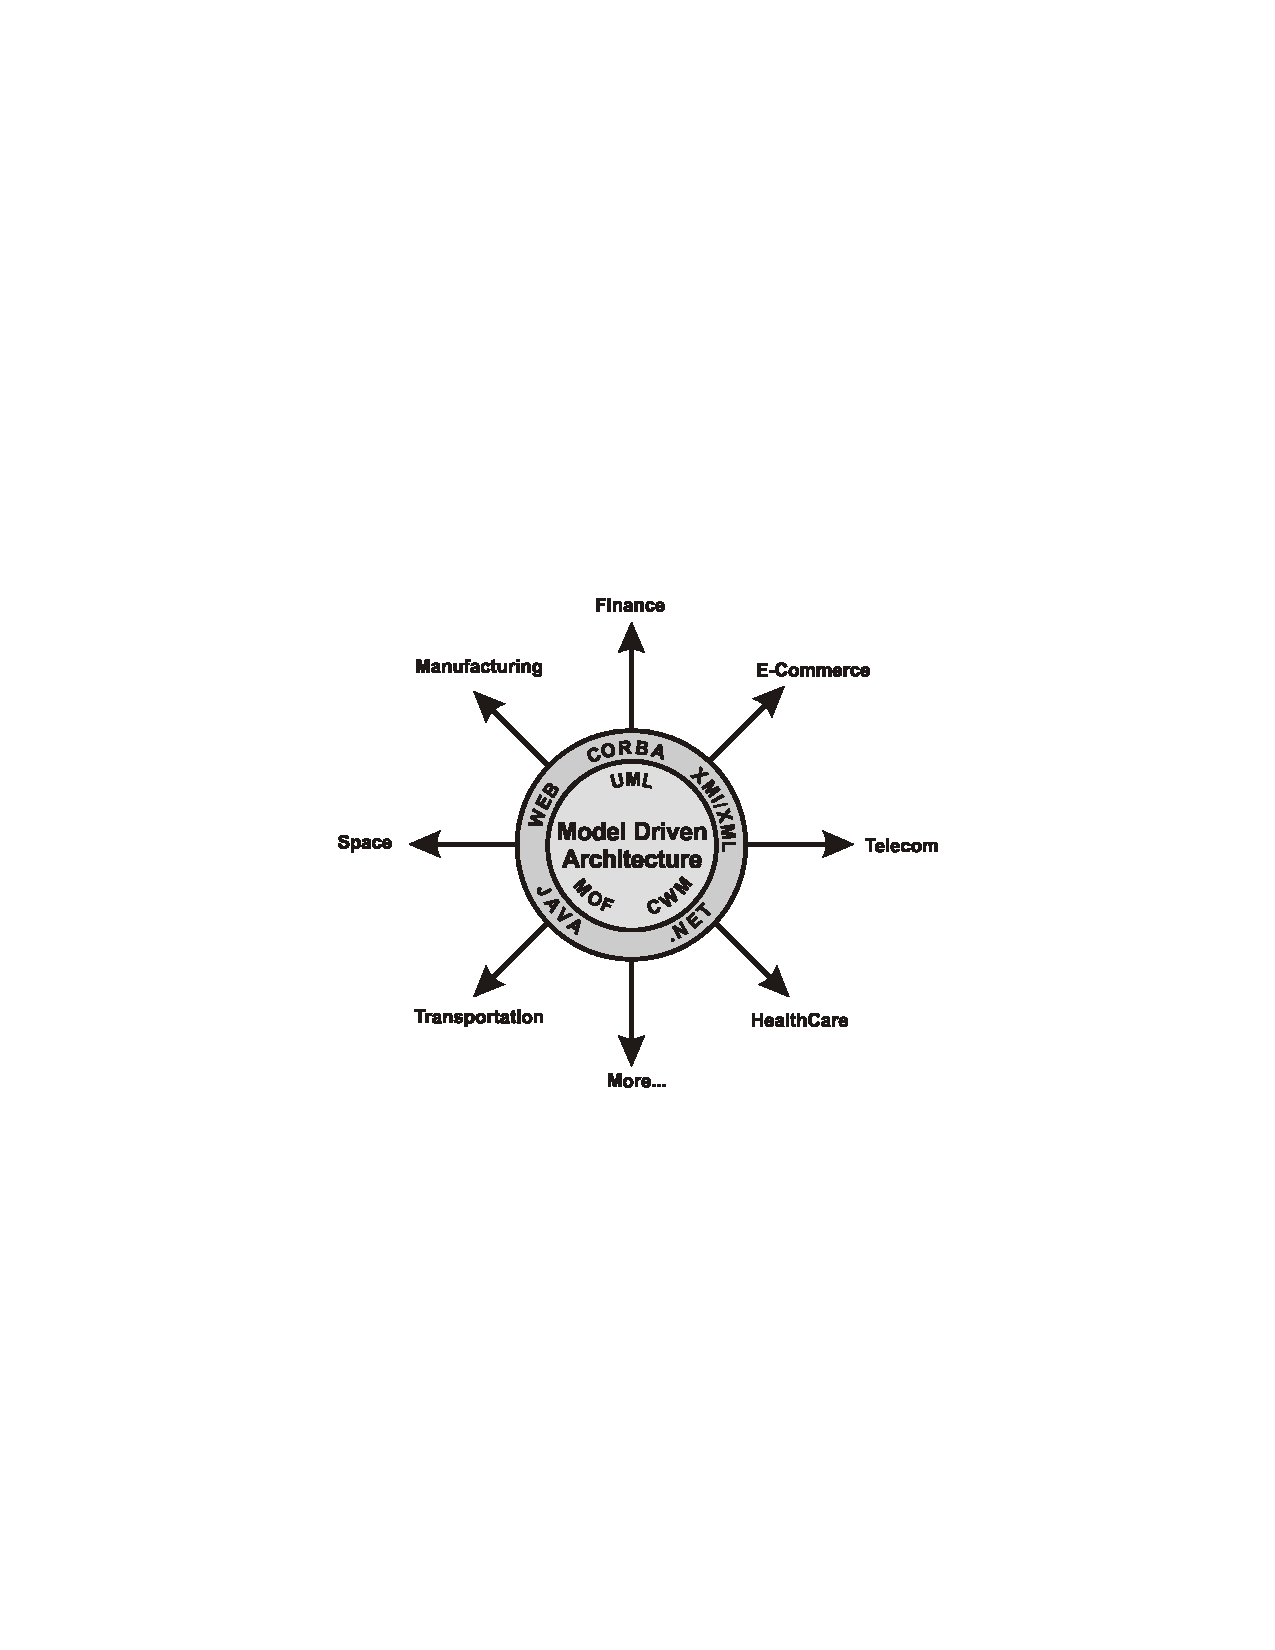
\includegraphics[width=0.8\hsize]{mda.pdf}
    \end{center}

\end{frame}

\begin{frame}
  \frametitle{模型转换: model transformation}
  \textbf{Model once, generate everywhere!} \\[2ex]
    %\begin{center}
      %\centering\includegraphics[width=0.9\hsize]{transform.pdf}
    %\end{center}

\noindent\begin{tikzpicture}[shorten >=1pt, auto, thick]
\tikzstyle{Process}=[draw=blue, rectangle, rounded corners, thick, fill=cyan!10, text width=1.6cm, align=center]

\tikzstyle{State}=[state, draw=none, fill=yellow!80, minimum width=1.2cm, circular drop shadow]

\node[Process] (Req) {需求分析} ;
\node[Process, right=of Req] (Ana) {系统分析} ;
\node[Process, right=of Ana] (Des) {设计} ;
\node[Process, right=of Des] (Pro) {编码} ;

\path [-Latex, thick, blue] (Req) edge [ dashed] (Ana)
    (Ana) edge (Des) 
    (Des) edge (Pro) ;

\node [State, below = 2 of Req] (CIM) {CIM} ;
\node [State, below = 2 of Ana] (PIM) {PIM} ;
\node [State, below = 2 of Des] (PSM) {PSM} ;
\node [State, below = 2 of Pro] (Code) {Code} ;

\path [->] (CIM) edge [loop below] node {0} () 
     edge [dashed] (PIM) 
    (PIM) edge [loop below] node {1} ()
     edge node [swap] {2} (PSM)  
    (PSM) edge [loop below] node {3} () 
      edge node [swap] {5} (Code) 
      edge [bend right=60] node {4} (PIM) 
    (Code) edge [loop below] node {6} ()
      edge [bend right=60] node {7} (PSM) ;
    
\end{tikzpicture}

\end{frame}

\begin{frame}
  \frametitle{OOA和OOD的MDA视图}
  \begin{columns}[c]
    \column{0.5\hsize}
    \begin{itemize}
      \item [OOA] 可得到一种平台无关的PIM模型
      \item [OOD] 可得到一种平台相关的PSM模型
\end{itemize}
    \column{0.5\hsize}
    \begin{center}
      \centering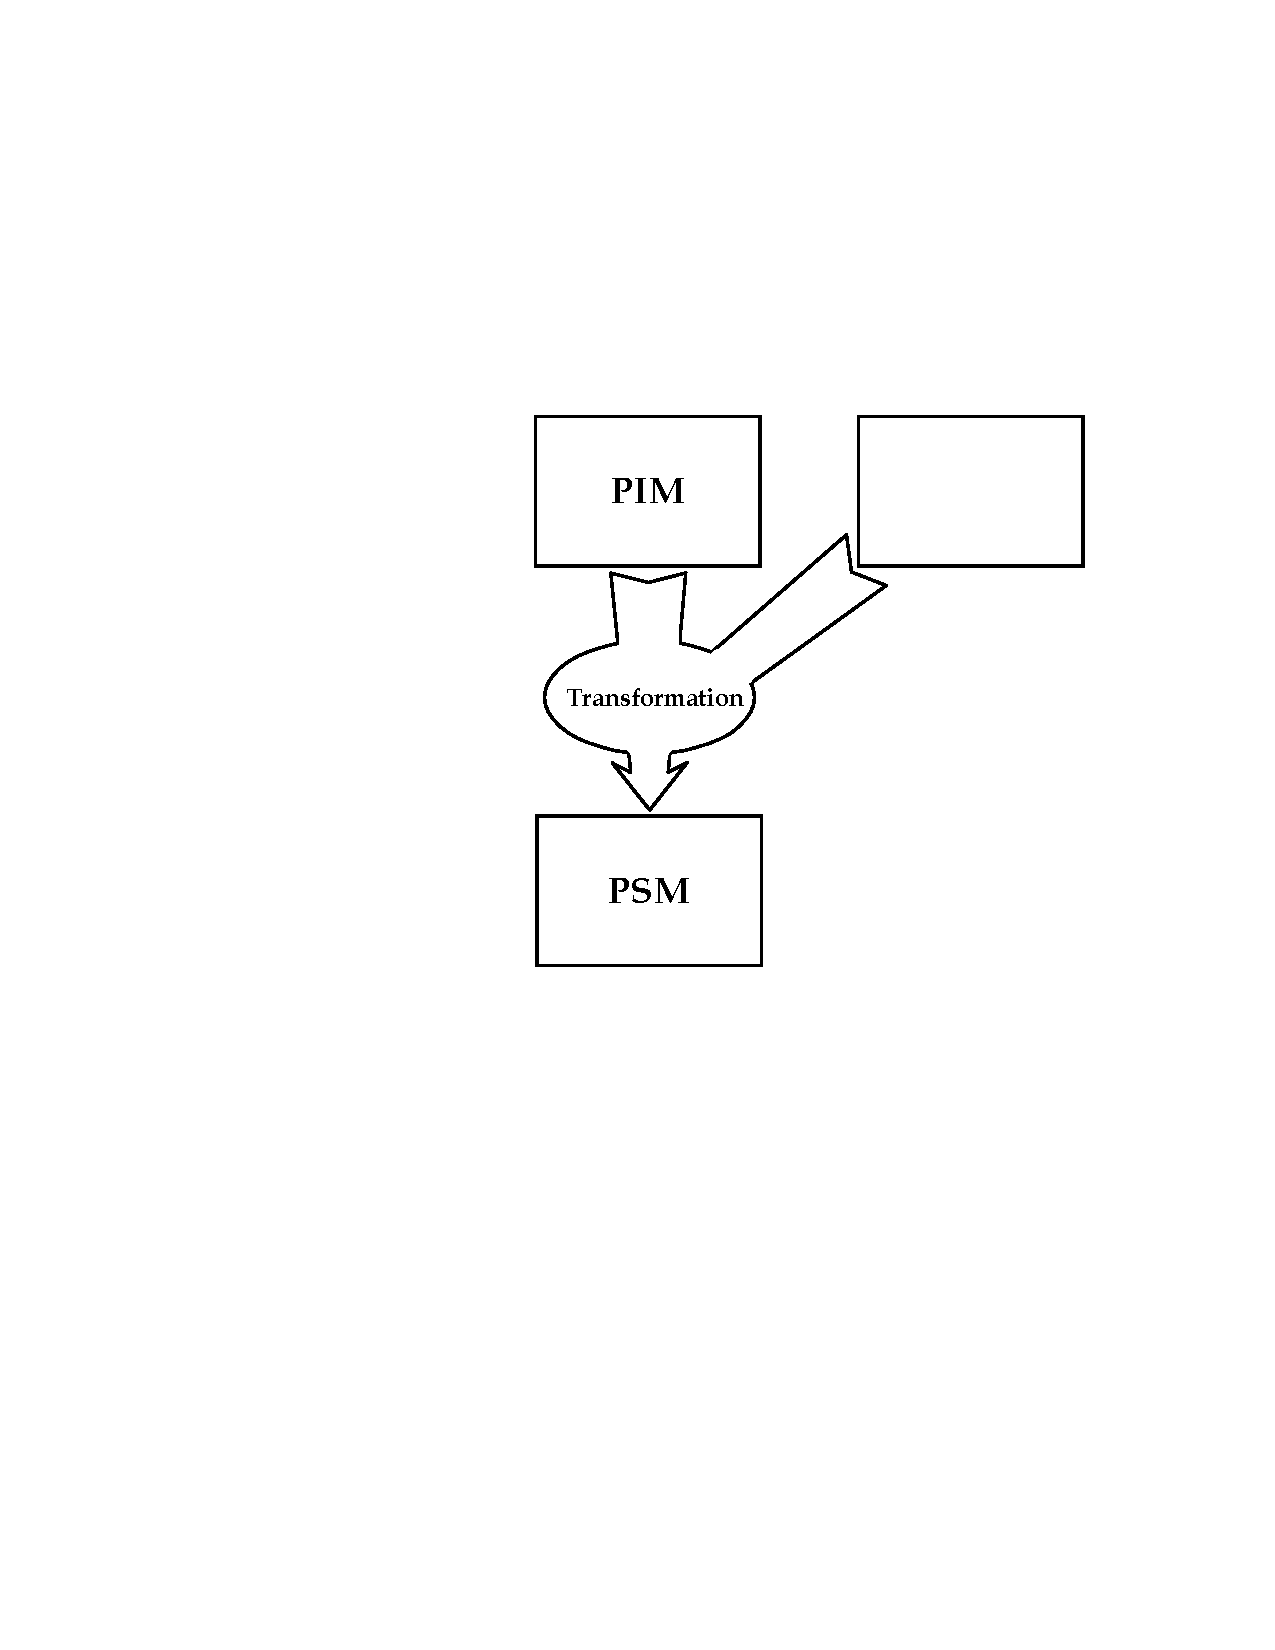
\includegraphics[width=0.8\hsize]{modeltrans.pdf}
    \end{center}
  \end{columns}
\end{frame}
\end{document}
